% 本文件是示例论文的一部分
% 本文是论文的第一章:绪论
% 论文的主文件是位于上级目录的 `main.tex`

\chapter{绪论}

\section{研究背景和意义}

西北地区由陕西、甘肃、宁夏、青海、新疆和内蒙古6省(区)组成,地域辽阔,人口相对稀少,该区气候干旱,降水稀少,蒸发旺盛,这样特殊的地理位置及气候条件决定了西北地区水资源短缺,生态环境脆弱。该区光热资源和土地、矿产资源比较丰富,属于资源开发主导型地区。然而,西北地区的水资源问题是该地区当前及未来国民经济和社会发展的最大制约因素,已引起了国家和社会的广泛关注\cite{黄智煌邬娜-2}。

西北地区气候干旱、降雨稀少,全区多年平均降水量2300mm,而水面蒸发量高达1000~2600mm以上,是全国唯一降水量极度少于农田作物和天然植被需水量的地区。据资料分析,西北地区多年平均地表水资源量约为1463亿立方米,地下水资源量998亿立方米,地下水资源与地表水资源重复计算量789亿立方米,水资源总量1672亿立方米,人均水资源总量2189立方米,耕地亩均水资源量857立方米。从表面上看,内陆河流域的人均、亩均水资源量并不算少,但由于水资源与人口、耕地的地区分布极不均衡,有相当大一部分分布在地势高寒、自然条件较差的人烟稀少地区及无人区,而自然条件较好、人口稠密、经济发达的绿洲地区水资源量十分有限。黄河流域河川径流具有地区分布不均、年际变化大及连续枯水等特点,内陆河流域的水资源主要以冰雪融水补给为主,年内分配高度集中,汛期径流量可占全年径流量的80%,部分河流汛期陡涨,枯季断流,开发利用的难度较大。\cite{仇巍巍陈从喜-1}


GIS 本质是运行在计算机上的一种软件,其是一门综合性的学科,集成应用了地理学、地图学、计算机科学、遥感学等,构建成一个集数据采集、存储、分析、显示、管理、计算等为一体的地理信息系统。该系统基于计算机运行,对地理空间信息进行分析并处理成图,将地表现象和事物可视化的显示出来。从以上的分析可以看出,其强大的功能适用于水文水资源领域,像调查地下水资源、地表水资源状况,以及监测水质与江河湖泊的水位变化等。GIS 技术在水文水资源领域的良好运用,对于水资源管理和保护工作有着重要意义。\cite{张国治韩景琦-3}

“雨水资源监控管理系统”是结合气象站、墒情站、GIS地理系统等监测传感设备,对于天气、墒情、地表水资源(包括水库、蓄水池、河流、地面径流雨水)等数据进行实施监测与传输,结合计算机软件,对于区域性雨水资源情况和用水结构进行协同管理,辅助当地政府和企业单位充分利用与开发当地雨水资源。\cite{郭明华-4}

GIS雨水资源专题图便是将区域性水资源,天气、墒情、地表水资源(包括水库、蓄水池、河流、地面径流雨水)等信息可视化,便于农户政府企业等对雨水等资源进行合理管理与利用来缓解西北地区用水资源短缺等问题,这对于西北地区发展资源开发,提高经济增长率,改善人民生活等具有重大的现实意义。\cite{刘治华-5}


\section{研究现状}
\subsection{国内研究现状}

现在针对西北地区的水资源现状,主要采取了如下对策:第一,强化水资源开发利用与保护的规划和监督管理,严格实施建设项目审批和管理制度。一方面,要制定出合理的水资源开发与保护方面的规划与制度,另一方面,要加强管理人员执法能力、技术能力等能力培养,加强执法必要设备的配置;第二,加强水利基本建设,如建设必要的调水工程,将部分水资源从富裕地区调往贫水区,或将优质水调往劣质水区,以改善缺水地区或不良水质地区的生产生活环境,也为生态环境建设提供必要的支持;第三,建设现代化的高效节水型经济社会,如适当提高水价,尤其是工业行业的水价,减少对水的浪费。发展集雨节灌,以解决农村用水困难,补充城市生态环境用水;第四,坚决实施有计划地退耕还林、还草。而且在西部大开发战略中,也水土资源的合理开发和有效利用摆在了更加突出的位置,而实现雨水资源的有效利用是水资源开发的一个主要方式,但是现在有关科研单位和水利部门的实现探索,主要是如何将雨水资源保存下来,发展雨水集蓄利用等技术,以及如何合理的使用雨水资源等技术的研究,但是没有将各个地区的雨水资源分布,受天气土地等影响因素导致的雨水收集效率等通过系统的方式形成系统性的可供各用水单位参考的资料等。
而通过GIS专题图便可以很好地实现各个地区的雨水资源分布的可视化系统,使得用水单位对雨水资源的调配等方面有系统的参考。

\subsection{国外研究现状}
地理信息系统(GIS)是以计算机为基础的综合处理和空间数据分析系统,是集计算机科学、管理科学、信息科学、地学等为一体的新兴边缘研究领域。20世纪70年代,美国田纳西河流域管理局利用GIS技术处理分析各种流域数据,为流域管理和规划提供决策服务,GIS便开始逐渐应用于水文水资源领域。80年代后随着计算机技术的飞速发展,GIS与水文水资源领域也有了广泛结合。

在国外,Gupta等早在1977年就实现了将栅格型GIS数据管理工具用于流域规划。随后欧洲一些研究机构也联合开发了具有水文过程模拟、水污染控制、水资源规划等功能的流域规划决策支持系统“WATERWARE”。近年Carlo等在GIS平台上开发了Ag-PIE模型,用于评价由于农业生产造成的地表和地下水水质下降的程度。

自20世纪70年代美国田纳西河流域管理局利用GIS技术处理和分析各种流域数据,开始为流域管理提供决策服务以来,GIS技术亦广泛应用于国外的水资源管理中。如美国科罗拉多州的一些机构联合开发了科罗拉多河决策支持系统,GIS被用于流域空间的存储、检索、分析和显示,以便于科罗拉多河水资源的管理。在灌区的水资源管理方面,位于美国德克萨斯州Lower Rio Grande Valley的8个灌区较早地开发以GIS为基础的灌区管理系统(DMS)。

 在国外,Davis曾将HEC-1、HEC-2与 GIS结合对洪水、水质和土坡侵蚀进行了模拟,可很好地用于洪灾损失评估。
 
 在国外,为了支持各种层次的水资源和水环境管理,美国国家环保局基于GIS技术和地调局水文数据开发了全美河段文件。He等将AGNPS、GRASS与GRASS Water Works模型集成在一起,综合评价了非点源污染对美国密歇根州Cass河水质的影响,近年来,Boyle等建立的IDOR2D系统将水污染模型与GIS集成。
 
 国外的分布式水文模型起始于1969年,比较著名的有TOPMODEL、SHE、IHDM模型和美国农业部的SWAT模型,目前得到了长足发展并在多个地区进行了实践和应用。近年出现的基于不规则三角网格(TIN)构建出得完全分布式模型,只需原始栅格节点的5%~10%就可以充分描述流域地形的水文特征,大大提高了分布式模型的计算效率,为大型流域的水文模拟提供了可能,是今后分布式水文模型研究的热点。国内的分布式水文模型研究起步较晚,沈晓东等在研究降雨和下垫面自然地理参数空间分布的不均匀性对径流过程的影响基础上,提出一个动态分布式降雨径流流域模型,实现了基于栅格DEM的坡面产汇流与河道汇流的数值模拟;郭生练等建立了一个基于DEM的分布式流域水文物理模型,用来模拟小流域的降雨径流时空变化过程;任立良等考虑了流域空间的变异性,基于DEM建立了参考作物蒸散量的分布式模型;李兰等在提出的变动生态产流模式的概念基础上建立了LL-I分布式降雨径流模型,能明显改善模拟预报精度,适合不同水文特征地区的产汇流计算
\section{主要工作}

雨水资源GIS专题图整体架构主要设计工作如下:
%使用{\nwafuthesis}模板排版学位论文的工作流如\ref{fig:workflow}所示。
%
%\begin{figure}[!htb]
%  \centering
%  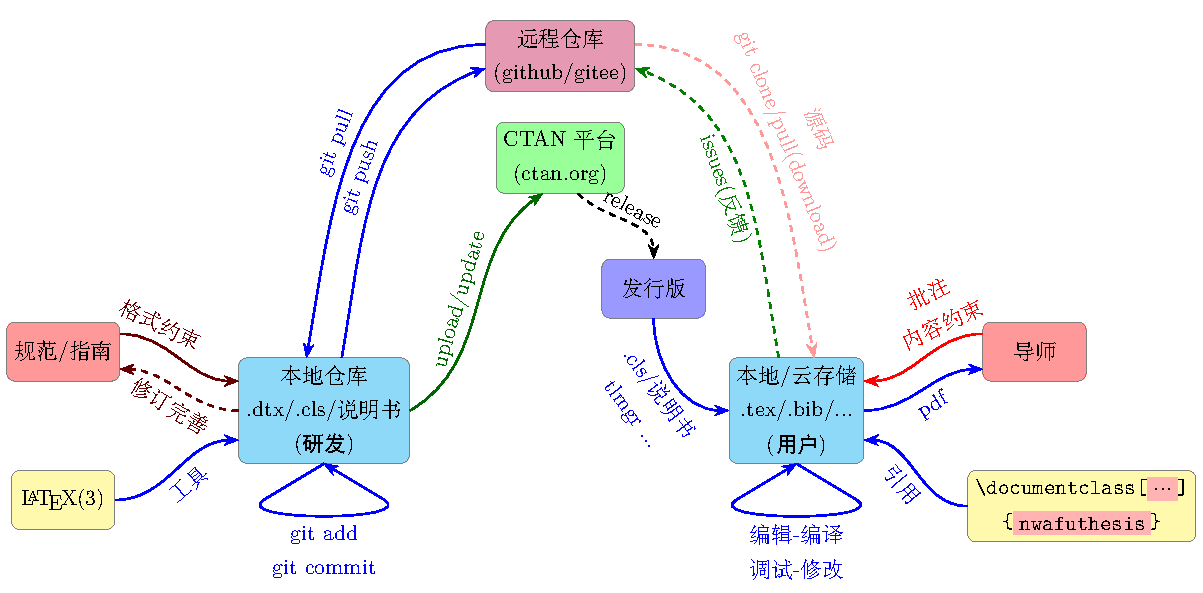
\includegraphics[width=0.85\textwidth]{figs/workflow}
%  \caption{模板工作流}
%  \label{fig:workflow}
%\end{figure}
\begin{enumerate}
	
\item 	数据设计:

GIS系统的数据按照性质的不同可以分为空间数据和属性数据,空间数据指地理空间对象的,属性数据包括地理空间对象的属性以及其他相关联的业务数据等。在了解GIS专题图在采集、存储、分析、研究、图示为一体的数据分析以及GIS专题图对于各种数据格式的定义等知识,GIS专题图的坐标系知识,为(历史、现在、未来)的水系信息,不同区域、时段等粒度的降雨信息,蒸散发信息,地下水信息,地形信息,不同区域粒度的土壤墒情,植被覆盖信息,光照、气温、降水信息,交通信息等为所需设计的雨水资源专题图设计合适的数据格式。
\item 	坐标系设计:

学习GIS专题图坐标系知识,结合系统需求分析以及与雨水资源各种元素因素特性,为雨水资源专题图中各种地形所需的不同的坐标系选择合适的坐标系。如图2所示。
\item	粒度设计

根据水资源不同元素因素的条件(历史、现在、未来)的水系信息,不同区域、时段等粒度的降雨信息,蒸散发信息,地下水信息,地形信息,不同区域粒度的土壤墒情,植被覆盖信息,光照、气温、降水信息等,设计不同时段区域类型等的粒度大小等信息。
\item	应用层设计

本系统的应用层主要是指IE,chrome,firhox等浏览器应用程序。本系统客户端设计采用“瘦客户端”的设计模式,即客户端无需安装任何插件即可进行地图的浏览、查询等操作,降低了对客户端配置的要求,减轻了客户端负担,用户只需普通IE等浏览器即可进行所有操作。本课题以AJAX技术为基础进行GIS专题图的开发,以XML作为与地图服务组件的数据传输协议。大大提升了系统的实用性和可扩展性等能力。
\item	基础底层设计

根据之前的坐标系设计,为不同坐标系下的数据信息设计各自的基础底层,例如地形信息需要基于海拔,地形3D信息的基础底层,而水资源分布只需基于平面的地图便可以表示。
\item 	影响因子设计

不同区域的水资源,如河流、水库、蓄水池、地下水、等水资源信息会受到各
种环境因素如,土壤类型,肥力,墒情,酸碱度,空气温湿度,分数,光照,
经纬度,海拔等因素影响,为了使得水资源信息更加准确,需要设计影响因子
作为水资源分布的参考要素。
\item 	操作图层设计

根据土壤墒情,植被覆盖信息,光照、气温、降水信息,地理信息等影响因子设计操作图层,使用户可以根据不同区域特定情况选择不同影响因子作用下的水资源分布,例如沙型土壤影响因子作用下的地下水的水资源较高,但是对于地表水资源便较少。

\item 	数据获取

采用ArcGIS Server服务,WMS(网络地图服务)、WFS(网络要素服务)等GIS数据服务以及ajax技术实现前后端数据通信,数据的获取。
\item 	数据可视化布局设计

使用OpenLayers和Pvechars库实现对应属性数据的可视化。编写代码实现研究内容中的各种GIS专题图,以及对GIS专题图和数据统计图进行整体组织和布局。
\end{enumerate}
\section{具体设计内容}

研究内容主要为雨水资源管理系统中的雨水资源GIS专题图的设计与实现。


1.	对水资源分布的历史、实时、未来等的信息按照不同的时段、区域、类型等粒度进行统计,并采用统计图(以及列表)的方式进行显示。


2.	水系信息的(历史、现在、未来)GIS专题图制作以及展示。

3.	不同区域、时段等粒度的降雨信息的(历史、现在、未来)GIS专题图制作以及展示。


4.	不同区域、时段、种植作物等粒度的蒸散发信息的(历史、现在、未来)GIS专题图制作以及展示。


5.	地下水信息的(历史、现在、未来)GIS专题图制作以及展示。


6.	地形信息的(历史、现在、未来)GIS专题图制作以及展示。

7.	不同区域粒度的土壤墒情之土壤类型、肥力、墒情、酸碱度等信息的(历史、现在、未来)GIS专题图制作以及展示。

8.	植被覆盖信息的(历史、现在、未来)GIS专题图制作以及展示。

9.	不同区域、时段等粒度的气候之光照、气温、降水等信息的(历史、现在、未来)GIS专题图制作以及展示。

10.	不同区域、时段等粒度的气候之光照、气温、降水等信息的(历史、现在、未来)GIS专题图制作以及展示。

11.	不同区域、时段等粒度的交通信息的GIS专题图制作以及展示。



\section{章节安排}
第一章和第二章主要是项目的主要设计内容,研究背景,研究现状以及实现技术等等,从第三章开始为项目的主体介绍,分为三章来介绍项目实现的成果,第三章主要是介绍本项目的需求分析,主要分为:功能需求,性能需求,界面需求,接口需求,第四章主要介绍雨水资源GIS专题图总体设计,主要为功能设计和数据库设计,第五章主要是介绍雨水资源专题图的详细设计与实现,主要为地表水系图,地下水系图,气候图。地表水系图分为河流水系图、蓄水池图、水库图、污水分布图等,地下水系图主要分为地下水分布图、土壤类型图、土壤含量图等,气候图则主要分为光照图、降雨图、温度图、风速风向图等。如\ref{fig:dirforest}所示。
\begin{figure}[!htb]%关于这些编译器的配置和使用,请参阅相关说明资料。
  \centering
  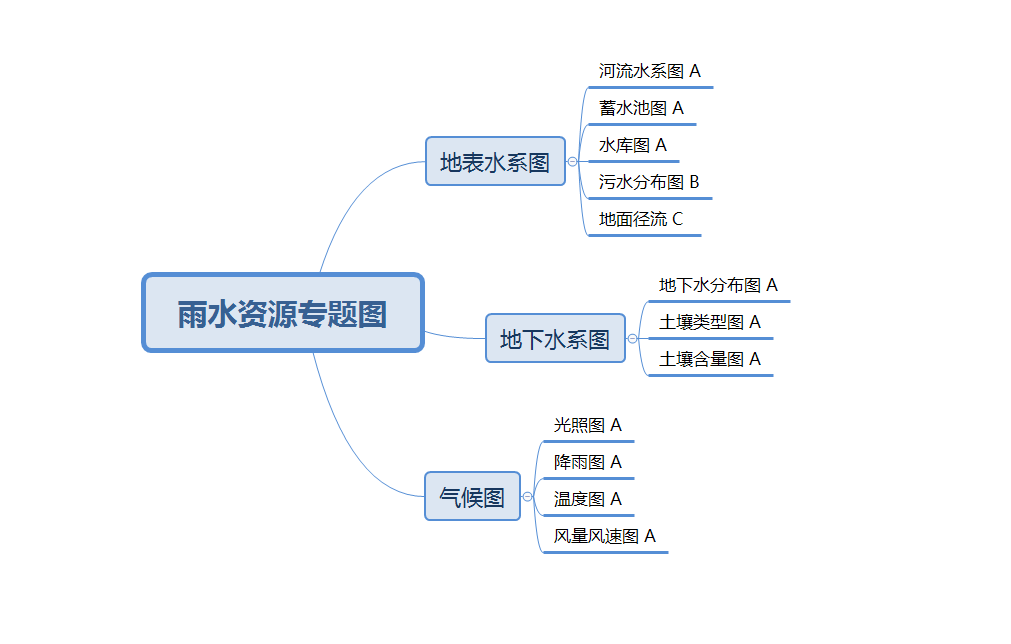
\includegraphics[width=0.60\textwidth]{figs/tree.png}
  \caption{雨水资源专题图分类}
  \label{fig:dirforest}
\end{figure}

%写作过程中的各个文件:
%

%完成部分或所有\verb|*.tex|撰写和修改后,可以在命令行使用 \verb|latexmk -xelatex main|
%进行编译输出\verb|main.pdf|文件,可以根据需要对结果\texttt{pdf}文件进行改名。
%
%也可以使用\texttt{TeXstudio}、\texttt{vscode}等GUI编辑器的进行编辑和编译输出。

%
%
%\note{}由于\nwafuthesis{}需要处理图、表、公式及参考文献等交叉引用,因此,
%往往需要多次编译才能得到正确的结果。为此,必须设置正确的编译方式和编译参数。
%关于多次编译的问题,大家可以浏览耿楠在B站发布的视频
%(\url{https://www.bilibili.com/video/BV1qa4y1v7my?spm_id_from=333.999.0.0})
%进行学习。



%如果论文需要双面打印的话,请务必修改文档类选项,编译双面打印用的 PDF 文件。
%具体地说,在主文件的头部,去除 \texttt{openany, oneside},
%改成 \texttt{twoside}。

%同时,建议注释\cs{nwafuset}命令中的\enquote{style/hyperlink = color},
%以\emph{取消超链接颜色}。

%%% Local Variables:
%%% mode: latex
%%% TeX-master: "../main.tex"
%%% End:
